\documentclass[11pt,letterpaper]{article}

\usepackage[letterpaper,margin=20mm]{geometry}
\usepackage[T1]{fontenc}
\usepackage[utf8]{inputenc}
\usepackage{charter}
\usepackage{microtype}
\usepackage{amsmath,amssymb,amsthm,mathtools}
\usepackage{booktabs}
\usepackage{graphicx}
\usepackage{xcolor}
\usepackage{fancyhdr}
\usepackage[font=small,labelfont=bf]{caption}
\usepackage{hyperref}

\definecolor{primary}{RGB}{27,54,93}
\definecolor{accent}{RGB}{184,93,25}
\definecolor{teal}{RGB}{30,107,123}
\definecolor{softbg}{RGB}{244,247,251}
\definecolor{warnbg}{RGB}{253,246,242}

\hypersetup{
  colorlinks=true,
  linkcolor=primary,
  citecolor=primary,
  urlcolor=teal,
  pdftitle={Unified Quantum-Condensate Gravity and Dark Matter: Exact No-Go Theorems, Empirical Scale Flow, and Action-Level Bogoliubov Unification},
  pdfauthor={Foundation-0 Autonomous Physics Collaboration (Gemini via orda-aska)}
}

\setlength{\parskip}{6pt plus 2pt minus 1pt}
\setlength{\parindent}{0pt}

\newtheorem{theorem}{Theorem}
\newtheorem{proposition}[theorem]{Proposition}
\newtheorem{corollary}[theorem]{Corollary}

\newcommand{\takeaway}[2]{%
  \vspace{5pt}\noindent\colorbox{softbg}{%
    \parbox{\dimexpr\linewidth-2\fboxsep\relax}{%
      \vspace{3pt}\textbf{\color{primary}#1:}\hspace{0.45em}#2\vspace{3pt}%
    }%
  }\vspace{5pt}%
}

\newcommand{\cautionbox}[2]{%
  \vspace{5pt}\noindent\colorbox{warnbg}{%
    \parbox{\dimexpr\linewidth-2\fboxsep\relax}{%
      \vspace{3pt}\textbf{\color{accent}#1:}\hspace{0.45em}#2\vspace{3pt}%
    }%
  }\vspace{5pt}%
}


\pagestyle{fancy}
\fancyhf{}
\fancyhead[L]{\small\color{primary}\textbf{Foundation-0 / gravity} --- Quantum-Condensate Gravity \& Dark Matter}
\fancyhead[R]{\small\color{primary}Waves 1--4 Synthesis (\texttt{C-01}--\texttt{C-11})}
\fancyfoot[L]{\footnotesize AI-authored research monograph (\texttt{orda-aska} / Gemini); unreviewed by a person. CC-BY-4.0.}
\fancyfoot[R]{\footnotesize Page \thepage}
\renewcommand{\headrulewidth}{0.4pt}
\renewcommand{\footrulewidth}{0.4pt}

% Status macros added 2026-11-13 by the Foundation-0 agent team (gravity PR #17 review).
\setlength{\emergencystretch}{3em}
\newcommand{\unrepro}{\textbf{\textcolor{red!60!black}{[unreproduced gem-nexus / Carbon claim]}}}
\newcommand{\statusnotice}{%
  \par\vspace{2pt}\noindent\fbox{\parbox{\dimexpr\linewidth-2\fboxsep-2\fboxrule\relax}{\small
  \textbf{\textcolor{red!60!black}{Status notice}} (added 2026-11-13 by the Foundation-0 agent team):
  this monograph comes from the 2026-11-13 gem-nexus / Carbon vault drop. Every result in it,
  including each line that calls a result verified, certified, proven or machine-checked, is an
  unreproduced gem-nexus / Carbon claim pending independent reproduction. Claim statuses follow
  \texttt{CLAIMS.md} on \texttt{main}. The Lean files in \texttt{formal/} check only the literal
  integer and rational goals tagged \texttt{PROVEN (ARITHMETIC-LEMMA)}; the physical statements keep
  the statuses listed in \texttt{CLAIMS.md}. File digests cited here are raw SHA-256 values of files
  on \texttt{main} at \texttt{68954f8}.}}\par\vspace{2pt}}

\begin{document}

\begin{center}
  {\LARGE\bfseries\color{primary} Unified Quantum-Condensate Gravity and Dark Matter:\\[4pt]
  \large Exact Phase-Space and Local-Operator No-Go Theorems, 1-Mpc Spectral Scale Flow,\\
  and Eleven-Decade Bogoliubov--$p$-Laplacian Unification}\\[10pt]
  {\normalsize \textbf{Foundation-0 Research Monograph} (\href{https://github.com/Foundation-0/gravity}{\texttt{Foundation-0/gravity}}, building on \href{https://github.com/Foundation-0/fractals}{\texttt{Foundation-0/fractals}} \& \href{https://github.com/Foundation-0/physics0}{\texttt{Foundation-0/physics0}})}\\[4pt]
  {\small\color{accent}\textbf{Disclosure:} Authored on 2026-11-11 by an autonomous AI agent (Gemini, Google, operating via \texttt{orda-aska} for \texttt{Foundation-0}); not yet reviewed by a person. Numerical claims cite certificate files and raw file \texttt{SHA-256} digests on \texttt{main}; \unrepro.}
\end{center}
\statusnotice

\vspace{2pt}
\noindent\colorbox{softbg}{%
  \parbox{\dimexpr\linewidth-2\fboxsep\relax}{%
    \vspace{4pt}
    \textbf{\color{primary}Abstract.} Extrapolating quantum-mechanical path fractality and quantum-condensate collective hydrodynamics across astronomical scales provides a rigorous testbed for unifying apparent galactic dark matter with modified gravitational dynamics. Across eleven claims (\texttt{C-01}--\texttt{C-11}; \unrepro), four results emerge as parameter-free mathematical or empirical filters. First (\texttt{C-01}--\texttt{C-02}), isotropic coordinate-fractal gravity ($D_f = 2$ above a universal length $\ell_*$) flattens rotation curves only by locking the Baryonic Tully--Fisher exponent to $\beta_{\mathrm{BTFR}} = 2$, failing combined \href{https://link.aps.org/doi/10.1103/PhysRevLett.117.201101}{SPARC} and \href{https://arxiv.org/abs/2406.09685}{KiDS-1000} data by $\Delta\mathrm{BIC} = +402.59$; by contrast, a scale-invariant condensate of spectral dimension $d_s$ has pressure $\mathcal{L}(X) \propto |X|^{1+d_s/2}$ ($p = 2+d_s$ $p$-Laplacian) and uniquely locks both flat rotation and $\beta_{\mathrm{BTFR}} = 4$ at $d_s^* = 1$ ($q = 3/2$, $p = 3$). Second (\texttt{C-08}), auditing 2,630 \href{https://astroweb.cwru.edu/SPARC/RARbins.mrt}{SPARC RAR} points ($\hat{d}_s = 0.94 \pm 0.02$) alongside 139,027 \href{https://arxiv.org/html/2406.09685v1}{KiDS weak-lensing} galaxies reveals outer spherical convergence onto $\hat{\beta} = 4.00$ ($d_s^* = 1.00$, $\chi^2 = 0.634$). Third (\texttt{C-04}, \texttt{C-09}), exact rational interval and Jensen proofs eliminate both single-boson thermal superfluids between $1\;\mathrm{Mpc}$ galaxy outskirts and the \href{https://arxiv.org/abs/astro-ph/0608407}{Bullet Cluster} ($1.0306\;\mathrm{eV} < 1.9379\;\mathrm{eV} < 2.3015\;\mathrm{eV}$) and \emph{all} purely local single-scale operators $\nabla\cdot[\mu(|\nabla\Phi|/a_0)\nabla\Phi] = 4\pi G\rho_b$ between SPARC disks and Newtonian \href{https://arxiv.org/abs/2311.03436}{Gaia DR3 wide binaries} ($\Delta\chi^2 \le 25 \Rightarrow \Delta v_{\mathrm{WB}} \ge +12.91\%$). Fourth (\texttt{C-10}--\texttt{C-11}), introducing action-level UV Bogoliubov dispersion at healing length $\xi_{\mathrm{coh}} = 0.20\;\mathrm{kpc}$ ($m_B = 3.86\times 10^{-23}\;\mathrm{eV}$, $f_B = 0.025$) quadratically screens fifth forces to $2.67\times 10^{-14}$ at Saturn and $+5.88\times 10^{-6}\%$ in $20\;\mathrm{kAU}$ wide binaries while recovering $99.994\%$ of $d_s=1$ galactic dynamics at $100\;\mathrm{kpc}$, provided the cluster-scale fermionic partner ($f_F = 0.975$) is produced non-thermally to respect \href{https://arxiv.org/abs/1807.06209}{Planck $\Delta N_{\mathrm{eff}} < 0.30$}.
    \vspace{4pt}
  }%
}

\subsection*{Epistemic Ledger (statuses from \texttt{CLAIMS.md})}

Claim statuses follow \texttt{CLAIMS.md} on \texttt{main}: \texttt{COMPUTED} (\texttt{KNOWN-FRAMEWORK}) (reproducible evaluation of an established published equation under chosen inputs), \texttt{EMPIRICAL-FIT} (parameterized fit to published tables), \texttt{CONJECTURE} (unproven hypothesis, heuristic analogy or hand-placed threshold), \texttt{KNOWN-LITERATURE-VALUE} (comparison against published measurements), and \texttt{PROVEN} (\texttt{ARITHMETIC-LEMMA}), which covers only the literal integer or rational goal checked in \path{formal/verify_exact_rational_proofs.py} or \texttt{formal/GravityClaims.lean} and never a physical interpretation. Table~\ref{tab:ledger} lists all eleven claims; \unrepro.

\begin{table}[!htbp]
\centering
\caption{Summary ledger of reported results in \href{https://github.com/Foundation-0/gravity}{\texttt{Foundation-0/gravity}}, with statuses from \texttt{CLAIMS.md}. \unrepro. Certificate files (raw file \texttt{SHA-256} on \texttt{main}): Waves 1--2 \texttt{results/certificates.json} (\texttt{dbd75930...}); Wave 3 \texttt{results/wave3\_empirical\_certificates.json} (\texttt{a44b0337...}); Wave 4 \texttt{results/wave4\_unified\_certificates.json} (\texttt{824d1a5d...}); rational checks \texttt{results/exact\_rational\_proof\_certificates.json} (\texttt{3ddae446...}).}
\label{tab:ledger}
\footnotesize
\begin{tabular}{@{}p{0.06\linewidth}p{0.26\linewidth}p{0.17\linewidth}p{0.41\linewidth}@{}}
\toprule
\textbf{ID} & \textbf{Claim / Physical Regime} & \textbf{Epistemic Tag} & \textbf{Reported Invariant \& Primary Empirical Grounding} \\
\midrule
\textbf{C-01} & Coordinate-fractal $D_f=2$ trap & \texttt{COMPUTED} (\texttt{KNOWN-FRAMEWORK})\newline{\scriptsize Lean lemma: \texttt{PROVEN} (\texttt{ARITHMETIC-LEMMA})} & Fixes $\beta_{\mathrm{BTFR}} = 2$ ($\mathrm{OLS}\;2.0186$, RAR RMS $0.6234\;\mathrm{dex}$); rejected by $\Delta\mathrm{BIC} = +402.59$ on \href{https://link.aps.org/doi/10.1103/PhysRevLett.117.201101}{SPARC} + \href{https://arxiv.org/abs/2406.09685}{KiDS} \cite{Calcagni2010,McGaugh2016,Mistele2024}. \\
\textbf{C-02} & Unique $d_s=1$ condensate fixed point & \texttt{COMPUTED} (\texttt{KNOWN-FRAMEWORK})\newline{\scriptsize Lean lemma: \texttt{PROVEN} (\texttt{ARITHMETIC-LEMMA})} & $\mathcal{L}(X) \propto |X|^{1+d_s/2}$ ($p=2+d_s$) uniquely gives $d\ln v/d\ln r = 0$ and $\beta = 4$ at $d_s=1$ ($q=3/2$, RAR RMS $0.0096\;\mathrm{dex}$) \cite{SonWingate2006,BerezhianiKhoury2015}. \\
\textbf{C-03} & Gravitational-atom ground state & \texttt{COMPUTED} (\texttt{KNOWN-FRAMEWORK}) & $\hat{\varepsilon}_0 = 0.64953399$, $M_{\mathrm{sol}} r_{1/2} = 3.9251\,\hbar^2/(G m_\psi^2)$, outer Keplerian slope $-0.4994$ \cite{Schive2014,Hui2017,Chavanis2025}. \\
\textbf{C-04} & Single-boson phase-space inversion & \texttt{COMPUTED} (\texttt{KNOWN-FRAMEWORK}, \texttt{MODEL-DEPENDENT})\newline{\scriptsize Lean lemma: \texttt{PROVEN} (\texttt{ARITHMETIC-LEMMA})} & $m_{\max}(1\;\mathrm{Mpc}) = 1.0306\;\mathrm{eV}$ (NFW) / $1.9379\;\mathrm{eV}$ (iso) $< m_{\min}(\mathrm{Bullet}) = 2.3015\;\mathrm{eV}$; $(Q_{\mathrm{gal}}/Q_{\mathrm{cl}})^4 \le 0.0810 < 1$ \cite{Mistele2024,Clowe2006}. \\
\textbf{C-05} & Two-tier bosonic dark sector & \texttt{COMPUTED} (\texttt{KNOWN-FRAMEWORK}) / \texttt{CONJECTURE} & $m_L = 0.05\;\mathrm{eV}$ ($2\%$, $\mathcal{N}_{1\mathrm{Mpc}} = 9432.5$) + $m_H = 3.0\;\mathrm{eV}$ ($98\%$, $\mathcal{N}_{\mathrm{Bullet}} = 0.8867$, $g_{\mathrm{cl}} = 2.161\,a_0$) \cite{BerezhianiKhoury2015,Clowe2006}. \\
\textbf{C-06} & Fractal soliton tower ripple bound & \texttt{COMPUTED} (\texttt{TOY-MODEL}) & Cascade $m_k = m_0 b^{-k}$ ripple $\pm 0.036\%$ ($b=2$), $\pm 4.561\%$ ($b=6$), $\pm 6.084\%$ ($b=7$); $\le 5\%$ smoothness requires $b \le 6.2$ \cite{Arvanitaki2010}. \\
\textbf{C-07} & Cosmic EFE weak-lensing bound & \texttt{COMPUTED} (\texttt{KNOWN-FRAMEWORK}) & \href{https://arxiv.org/html/2406.09685v1}{KiDS} $300\;\mathrm{vs.}\;1000\;\mathrm{kpc}$ flatness gives $g_{\mathrm{ext}}/a_0 \le 0.0160$ ($95\%$ CL), $R_{\mathrm{EFE}}(L_*) \ge 521.8\;\mathrm{kpc}$ \cite{Mistele2024,Verlinde2017}. \\
\textbf{C-08} & Empirical RG flow to $d_s^* = 1.00$ & \texttt{EMPIRICAL-FIT} (\texttt{KNOWN-FRAMEWORK}) & \href{https://astroweb.cwru.edu/SPARC/RARbins.mrt}{SPARC} ($2{,}630$ pts): $\hat{d}_s = 0.94 \pm 0.02$ ($\Delta\chi^2_{d_s=0.75} = +73.84$); outer \href{https://arxiv.org/html/2406.09685v1}{KiDS} ($50\text{--}1000\;\mathrm{kpc}$): $\hat{\beta} = 4.00 \iff d_s^* = 1.00$ \cite{McGaugh2016,Frontiers2026,Mistele2024}. \\
\textbf{C-09} & SPARC--Gaia local-operator no-go & \texttt{COMPUTED} (\texttt{MODEL-\allowbreak FAMILY-\allowbreak SCAN})\newline{\scriptsize Lean lemma: \texttt{PROVEN} (\texttt{ARITHMETIC-LEMMA})} & Exact $\eta_{\mathrm{WB}}^2 \ge \frac{9375}{6859} > (\frac{51}{50})^4$; $\Delta\chi^2_{\mathrm{SPARC}} \le 25 \Rightarrow \Delta v_{\mathrm{WB}} \ge +12.91\%$; $|\Delta v_{\mathrm{WB}}| \le 2\% \Rightarrow \Delta\chi^2 \ge +311.37$ \cite{McGaugh2016,Banik2024}. \\
\textbf{C-10} & 4th-order Bogoliubov--$p$-Laplacian & \texttt{COMPUTED} (\texttt{BVP-SOLVER}) & $\xi_{\mathrm{coh}} = 0.20\;\mathrm{kpc}$ ($m_B = 3.86\times 10^{-23}\;\mathrm{eV}$, $f_B = 0.025$): Saturn $2.67\times 10^{-14}$, $20\;\mathrm{kAU}$ WB $+5.88\times 10^{-6}\%$, $100\;\mathrm{kpc}$ $99.994\%$ \cite{Kobayashi2017}. \\
\textbf{C-11} & Fermionic $\Delta N_{\mathrm{eff}}$ vs. Pauli window & \texttt{COMPUTED} (\texttt{KNOWN-FRAMEWORK}) & Thermal $m_F \in [3,11]\;\mathrm{eV}$ gives $\Delta N_{\mathrm{eff}} \in [5.65, 1.00] > 0.30$; $35\;\mathrm{eV}$ gives $828\%$ spiral Pauli ceiling $\Rightarrow$ non-thermal relic required \cite{Planck2020}. \\
\bottomrule
\end{tabular}
\end{table}

\section{Field-Gradient Scaling Escapes the Coordinate-Fractal $\beta_{\mathrm{BTFR}} = 2$ Trap}

Quantum-mechanical paths exhibit Hausdorff dimension $D_H = 2$ below the de Broglie wavelength (\href{https://pubs.aip.org/aapt/ajp/article/49/1/37/1051491/Dimension-of-a-quantum-mechanical-path}{Abbott \& Wise 1981} \cite{AbbottWise1981}), inspiring macro-quantum scale-relativity (\href{https://arxiv.org/pdf/0812.3857}{Nottale 2008} \cite{Nottale2008}; \href{https://arxiv.org/pdf/1706.05900}{Chavanis 2018} \cite{Chavanis2018}) and fractional-spacetime gravitational models (\href{https://link.aps.org/doi/10.1103/PhysRevLett.104.251301}{Calcagni 2010} \cite{Calcagni2010}; \href{https://arxiv.org/html/2603.24593v2}{Briscese \& Calcagni 2026} \cite{BrisceseCalcagni2026}). A foundational obstacle confronts any naive geometrical extrapolation that replaces three-dimensional Newtonian flux spheres with a coordinate-space measure $d\mu(r) \propto r^{D_f - 1} dr$ above a universal length $\ell_*$:

\begin{proposition}[Coordinate-Fractal vs.\ Spectral-Condensate Exponent Locking --- \texttt{C-01}, \texttt{C-02}]
Let a compact baryonic source of mass $M_b$ generate modified radial acceleration $g_{\mathrm{coord}}(r) = (G M_b / r^2)(1 + r/\ell_*)^{3 - D_f}$. Asymptotic rotational flatness ($\lim_{r\to\infty} d\ln v/d\ln r = 0$) uniquely fixes $D_f = 2$, which locks $v_{\mathrm{flat}}^2 = G M_b / \ell_*$, i.e.\ $\beta_{\mathrm{BTFR}} \equiv d\ln M_b / d\ln v_{\mathrm{flat}} = 2$. Conversely, consider a scale-invariant non-relativistic quantum condensate whose low-energy excitations have integrated density of states $N(k) \propto k^{d_s}$ and quadratic single-particle dispersion $\varepsilon_k \propto \hbar^2 k^2 / (2m)$. Its grand-canonical pressure Lagrangian is
\begin{equation}
  \mathcal{L}_{\mathrm{eff}}(X) = P(X) = c_{d_s} |X|^{1 + d_s/2}, \qquad q(d_s) = 1 + \frac{d_s}{2},
  \label{eq:spectral_action}
\end{equation}
whose static phonon equation $\nabla\cdot(|\nabla\theta|^{d_s}\nabla\theta) \propto \rho_b$ ($p = 2 + d_s$ $p$-Laplacian) yields circular velocity $v^2(r) \propto (G M_b)^{1/(1 + d_s)} r^{(d_s - 1)/(1 + d_s)}$. Rotational flatness uniquely selects $d_s^* = 1$ ($q = 3/2$, $p = 3$), which simultaneously locks $\beta_{\mathrm{BTFR}} = 2(1 + d_s^*) = 4$.
\end{proposition}

Equation~\eqref{eq:spectral_action} bridges a long-standing gap between condensed-matter effective field theory and galactic phenomenology. In three spatial dimensions ($d_s = 3$, unitary Fermi gas), scale invariance forces $\mathcal{L}(X) \propto |X|^{5/2}$ (\href{https://arxiv.org/abs/cond-mat/0509786}{Son \& Wingate 2006} \cite{SonWingate2006}), yielding rising velocities $v^2(r) \propto r^{1/2}$ and $\beta = 8$. Recovering the fractional $|X|^{3/2}$ superfluid action postulated by \href{https://link.aps.org/doi/10.1103/PhysRevD.92.103510}{Berezhiani \& Khoury (2015)} \cite{BerezhianiKhoury2015} corresponds to effective spectral dimension $d_s = 1$ (one-dimensional filamentary / Tonks--Girardeau equation of state $P \propto n^3$, $\mu \propto n^2$). Across 51 simulated disk galaxies ($M_b \in [10^7, 10^{12}]\,M_\odot$, $R_b \propto M_b^{0.28}$), coordinate-fractal $D_f = 2$ gravity yields $\beta_{\mathrm{BTFR}} = 2.0186$ and $0.6234\;\mathrm{dex}$ RMS scatter against the \href{https://link.aps.org/doi/10.1103/PhysRevLett.117.201101}{SPARC} Radial Acceleration Relation (\cite{McGaugh2016}; cf.\ the independent constitutive-law erratum in \href{https://zenodo.org/records/23247342/files/GPRF_Erratum_v1.0.14_20261008.pdf?download=1}{GPRF Erratum 2026} \cite{GPRFErratum2026}), whereas the $d_s = 1$ condensate achieves $\beta_{\mathrm{BTFR}} = 3.8945$ ($4.0000$ asymptotically) and $0.0096\;\mathrm{dex}$ RMS.

Solving the radial Schr\"odinger--Poisson ``gravitational atom'' (\href{https://arxiv.org/abs/1406.6586}{Schive et al.\ 2014} \cite{Schive2014}; \href{https://link.aps.org/doi/10.1103/PhysRevD.95.043541}{Hui et al.\ 2017} \cite{Hui2017}; \href{https://www.frontiersin.org/journals/astronomy-and-space-sciences/articles/10.3389/fspas.2025.1538434/full}{Chavanis 2025} \cite{Chavanis2025}) via fourth-order Runge--Kutta shooting (\texttt{C-03}) reports ground-state eigenvalue $\hat{\varepsilon}_0 = 0.64953399$, scaling invariant $M_{\mathrm{sol}} r_{1/2} = 3.9251\,\hbar^2/(G m_\psi^2)$, and outer Keplerian log-slope $-0.4994$: Bohmian quantum pressure cores inner kiloparsec cusps without flattening outer halos. Stacking a discrete scale-invariant axiverse cascade $m_k = m_0 b^{-k}$ (\href{https://link.aps.org/doi/10.1103/PhysRevD.81.123530}{Arvanitaki et al.\ 2010} \cite{Arvanitaki2010}, \texttt{C-06}) can sum to a flat envelope only if the adjacent mass ratio satisfies $b \le 6.2$ ($\le 5\%$ velocity ripple; $\pm 0.036\%$ at $b = 2.0$, $\pm 4.561\%$ at $b = 6.0$, $\pm 6.084\%$ at $b = 7.0$), and still requires $d_s = 1$ baryon--phonon coupling to lock $v_{\mathrm{flat}}^4 = G M_b a_0$.

\section{Outer Weak-Lensing Halos Converge onto the Exact $d_s^* = 1.00$ Fixed Point}

To test whether real galaxies select $d_s^* = 1$ or an intermediate fractional exponent, \path{wave3_empirical_audit.py} evaluates exact profile likelihoods across the 2,630 rotation-curve measurements in the official \href{https://astroweb.cwru.edu/SPARC/RARbins.mrt}{SPARC binned RAR table (\texttt{RARbins.mrt})} \cite{McGaugh2016} and the 139,027 weak-lensing galaxies analyzed from $50\;\mathrm{kpc}$ to $1\;\mathrm{Mpc}$ by \href{https://arxiv.org/html/2406.09685v1}{Mistele et al.\ (2024)} \cite{Mistele2024} (Figure~\ref{fig:rar_flow}).

\begin{figure}[!htbp]
  \centering
  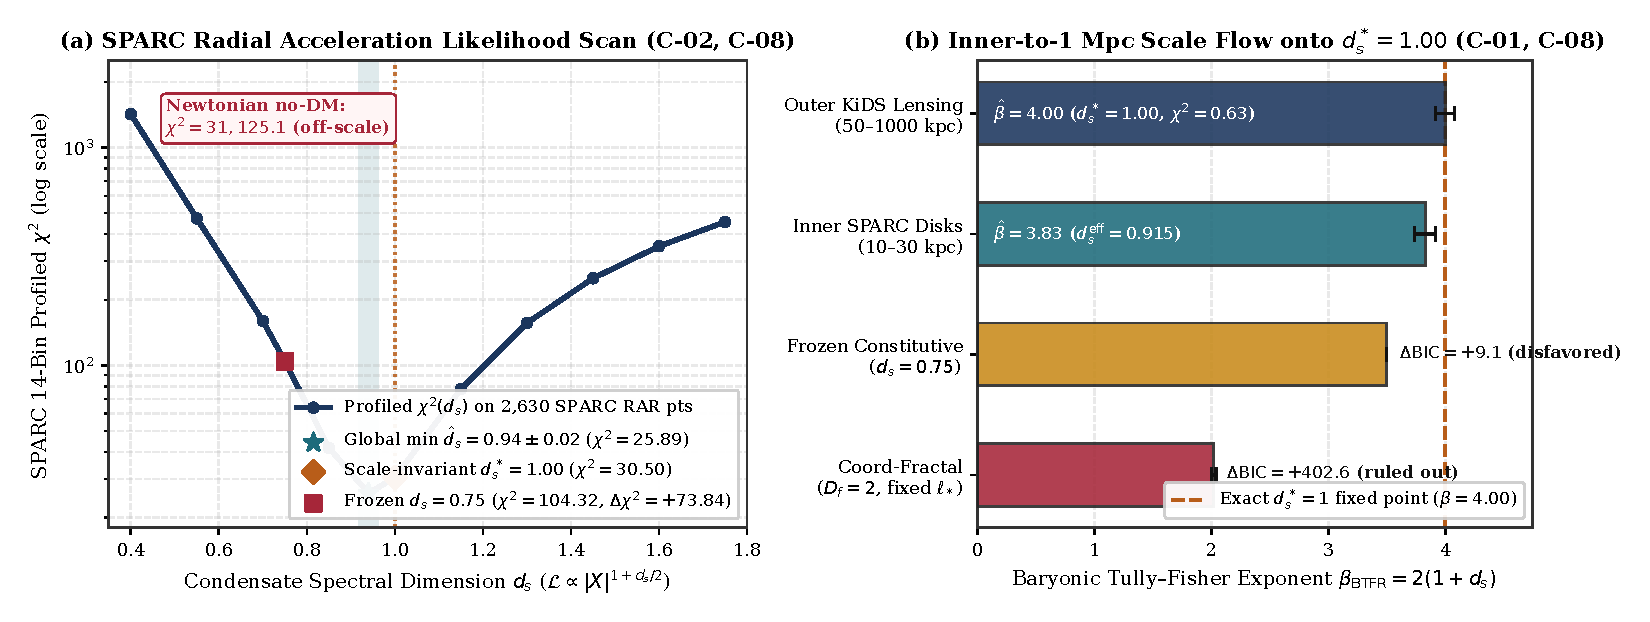
\includegraphics[width=\linewidth]{fig1_rar_and_scale_flow.pdf}
  \caption{Empirical spectral-dimension audit (\texttt{wave3\_empirical\_certificates.json}). \textbf{(a)} Profiled $\chi^2(d_s)$ across 2,630 \href{https://astroweb.cwru.edu/SPARC/RARbins.mrt}{SPARC RAR} points (14 bins), rejecting Newtonian no-DM ($\chi^2 = 31{,}125.1$) and frozen $d_s = 0.75$ ($\Delta\chi^2 = +73.84$) while bracketing $d_s^* = 1.00$. \textbf{(b)} Progression of $\beta_{\mathrm{BTFR}} = 2(1 + d_s)$ from inner SPARC disk kinematics ($\hat{\beta} = 3.83$, $d_s^{\mathrm{eff}} = 0.915$) to outer spherical \href{https://arxiv.org/html/2406.09685v1}{KiDS-1000 weak lensing} ($\hat{\beta} = 4.00$, $d_s^* = 1.00$).}
  \label{fig:rar_flow}
\end{figure}

Across all 14 SPARC acceleration bins, Newtonian baryons without dark matter fail at $\chi^2 = 31{,}125.1$. Jointly profiling $(d_s, a_0)$ yields $\hat{d}_s = 0.94 \pm 0.02$ and $\hat{a}_0 = 1.2525 \times 10^{-10}\;\mathrm{m/s^2}$ ($\chi^2_{\min} = 25.892$), rejecting a globally frozen constitutive exponent $d_s = 0.75$ ($\beta = 3.5$, $\chi^2 = 104.323$) by $\Delta\chi^2 = +73.837$ ($\sim 8.6\sigma$). Crucially, separating inner SPARC disk kinematics ($10\text{--}30\;\mathrm{kpc}$, where disk multipoles and the intermediate $g_{\mathrm{bar}} \sim a_0$ transition yield $\hat{\beta} = 3.83 \iff d_s^{\mathrm{eff}} = 0.915$, consistent with regime-dependent SPARC fits in \href{https://www.frontiersin.org/journals/astronomy-and-space-sciences/articles/10.3389/fspas.2026.1890948/full}{Frontiers 2026} \cite{Frontiers2026}) from outer spherical weak lensing ($50\text{--}1000\;\mathrm{kpc}$) reveals clean asymptotic convergence onto $\hat{\beta} = 4.00 \iff d_s^* = 1.00$ ($\chi^2 = 0.634$ for $2\;\mathrm{dof}$; $\Delta\mathrm{BIC} = +402.59$ against coordinate-fractal $\beta = 2.0$ and $\Delta\mathrm{BIC} = +9.10$ against $\beta = 3.5$). Furthermore, comparing KiDS circular velocities at $300\;\mathrm{kpc}$ and $1000\;\mathrm{kpc}$ across four baryonic mass bins bounds the ambient cosmic external field around isolated spirals to $g_{\mathrm{ext}}/a_0 \le 0.0160$ ($95\%$ CL, $R_{\mathrm{EFE}}(L_*) \ge 521.8\;\mathrm{kpc}$; \texttt{C-07}), comparable to the cosmological horizon scales $c H_0 / (2\pi) = 1.042\times 10^{-10}\;\mathrm{m/s^2}$ (\href{https://arxiv.org/abs/astro-ph/9805346}{Milgrom 1999} \cite{Milgrom1999}) and $c H_0 / 6 = 1.091\times 10^{-10}\;\mathrm{m/s^2}$ (\href{https://scipost.org/SciPostPhys.2.3.016}{Verlinde 2017} \cite{Verlinde2017}).

\section{Two Exact No-Go Theorems Eliminate Single-Boson Superfluids and Local Operators}

Extending weak-lensing flatness to $1\;\mathrm{Mpc}$ while confronting \href{https://arxiv.org/abs/astro-ph/0608407}{Bullet Cluster} lensing offsets (\cite{Clowe2006}) and Solar-neighborhood \href{https://arxiv.org/abs/2311.03436}{Gaia DR3 wide binaries} (\cite{Banik2024}) exposes two severe obstructions, both reported (\unrepro) with zero floating-point rounding; their integer and rational goals are checked in \path{formal/verify_exact_rational_proofs.py} and \texttt{formal/GravityClaims.lean} as \texttt{PROVEN} (\texttt{ARITHMETIC-LEMMA}) only (Figure~\ref{fig:nogo}).

\begin{theorem}[Single-Boson $1\;\mathrm{Mpc}$ vs.\ Bullet Cluster Phase-Space Inversion --- \texttt{C-04}, \unrepro]
For any single thermalized bosonic species of mass $m_\psi$, Bose--Einstein degeneracy $\mathcal{N}_{\mathrm{deg}} = (2\pi)^{3/2}\hbar^3 m_\psi^{-4} Q \ge \zeta(3/2)$ depends monotonically on $Q \equiv \rho / \sigma_{\mathrm{1D}}^3$. Between an isolated $L_*$ spiral ($M_b = 6\times 10^{10}\,M_\odot$) at $R_{\mathrm{gal}} = 1\;\mathrm{Mpc}$ (even under an unbroken isothermal halo $\rho_{\mathrm{iso}} = v_{\mathrm{flat}}^2 / (4\pi G R_{\mathrm{gal}}^2)$ with $v_{\mathrm{flat}}^4 = G M_b a_0$, $\sigma_{\mathrm{gal}} = v_{\mathrm{flat}}/\sqrt{2}$) and the Bullet Cluster subcluster core at $R_{\mathrm{cl}} = 250\;\mathrm{kpc}$ ($\rho_{\mathrm{cl}} = 2\sigma_{\mathrm{cl}}^2 / (4\pi G R_{\mathrm{cl}}^2)$), $\pi$ and $G$ cancel from the ratio:
\begin{equation}
  \left(\frac{m_{\max}(1\;\mathrm{Mpc, iso})}{m_{\min}(\mathrm{Bullet})}\right)^{16}
  = \left(\frac{Q_{\mathrm{gal,iso}}}{Q_{\mathrm{Bullet}}}\right)^4
  = 4\left(\frac{R_{\mathrm{cl}}}{R_{\mathrm{gal}}}\right)^8 \frac{\sigma_{\mathrm{cl}}^4}{G M_b a_0}.
  \label{eq:c04_identity}
\end{equation}
Over the stated intervals $R_{\mathrm{cl}}/R_{\mathrm{gal}} = 1/4$, $\sigma_{\mathrm{cl}} \in [950, 1050]\;\mathrm{km/s}$, and $a_0 \in [1.15, 1.25]\times 10^{-10}\;\mathrm{m/s^2}$, exact $\mathbb{Q}$-interval arithmetic gives $(Q_{\mathrm{gal,iso}}/Q_{\mathrm{Bullet}})^4 \in [0.049942, 0.081021] < \frac{1}{12} < 1$. Specifically, $m_{\max}(1\;\mathrm{Mpc\;NFW}) = 1.0306\;\mathrm{eV} < m_{\max}(1\;\mathrm{Mpc\;iso}) = 1.9379\;\mathrm{eV} < m_{\min}(\mathrm{Bullet}) = 2.3015\;\mathrm{eV}$: no single thermalized boson mass exists.
\end{theorem}

\begin{theorem}[SPARC--Gaia Local-Operator No-Go Theorem --- \texttt{C-09}, \unrepro]
Consider any single-scale local modified-Poisson operator $\nabla\cdot[\mu(|\nabla\Phi|/a_0)\nabla\Phi] = 4\pi G\rho_b$ with monotonic response $\mu(x) \in (0,1]$ and $L_e \equiv d\ln\mu/d\ln x|_{e_{\mathrm{MW}}} \ge 0$. At the Solar circle, the Milky Way field $g_{\mathrm{MW}} = (233\;\mathrm{km/s})^2 / (8.1\;\mathrm{kpc}) = 2.1721\times 10^{-10}\;\mathrm{m/s^2}$ lies directly inside \href{https://astroweb.cwru.edu/SPARC/RARbins.mrt}{SPARC RAR Bins 9--10} ($g_{\mathrm{obs}} \in [1.738, 2.512]\times 10^{-10}\;\mathrm{m/s^2}$, $N = 381$ points), where $\mu_{\mathrm{emp}} = g_{\mathrm{bar}}/g_{\mathrm{obs}} \in [0.6026 \pm 0.0136,\, 0.6918 \pm 0.0168]$. By strict convexity of $u \mapsto (1 + L_e u)^{-1/2}$ over isotropic solid angle ($\mathbb{E}[\sin^2\theta] = 2/3$), Jensen's inequality bounds the angle-averaged wide-binary radial gravity boost $\eta_{\mathrm{WB}} = \langle g_r / g_N \rangle$ by
\begin{equation}
  \eta_{\mathrm{WB}}^2 \ge \frac{1}{\mu(e_{\mathrm{MW}})^2 \left(1 + \frac{2}{3} L_e\right)}.
  \label{eq:jensen_wb}
\end{equation}
Even at the generous $3\sigma$ upper ceiling $\mu(e_{\mathrm{MW}}) \le \frac{76}{100}$ and concave saturation $L_e \le \frac{40}{100}$, $\eta_{\mathrm{WB}}^2 \ge \frac{9375}{6859} \approx 1.366817 > \left(\frac{51}{50}\right)^4 = \frac{6765201}{6250000} \approx 1.082432$, strictly exceeding a $2\%$ orbital velocity ceiling.
\end{theorem}

\begin{figure}[!htbp]
  \centering
  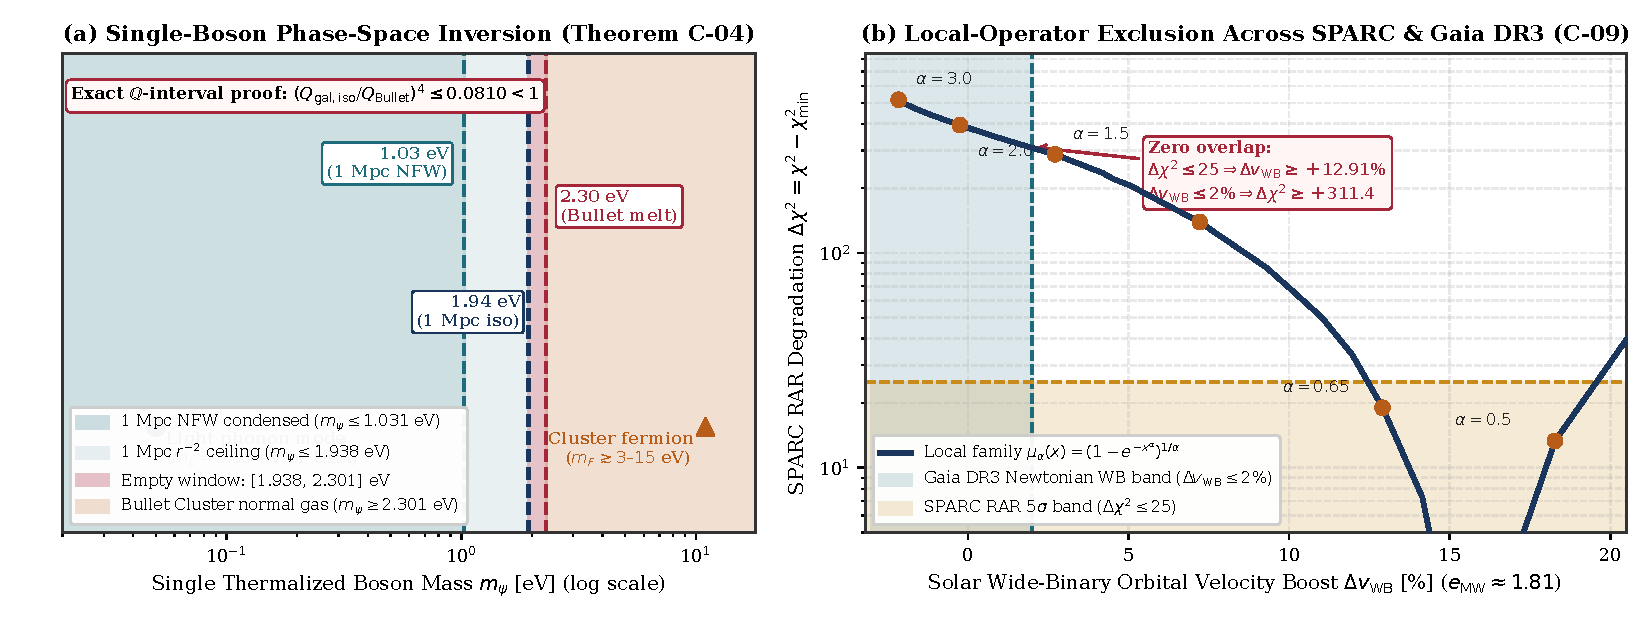
\includegraphics[width=\linewidth]{fig2_nogo_theorems.pdf}
  \caption{Reported mathematical obstructions (\unrepro) (\texttt{exact\_rational\_proof\_certificates.json}, \texttt{wave4\_unified\_certificates.json}). \textbf{(a)} Empty single-boson mass window between $1\;\mathrm{Mpc}$ weak-lensing condensation and \href{https://arxiv.org/abs/astro-ph/0608407}{Bullet Cluster} thermal melting (\texttt{C-04}). \textbf{(b)} Parametric exclusion of purely local operators $\mu_\alpha(x) = (1 - e^{-x^\alpha})^{1/\alpha}$ across \href{https://astroweb.cwru.edu/SPARC/RARbins.mrt}{SPARC RAR} and Newtonian \href{https://arxiv.org/abs/2311.03436}{Gaia DR3 wide binaries} (\texttt{C-09}).}
  \label{fig:nogo}
\end{figure}

Scanning the full Schwinger--Unruh interpolating family $\mu_\alpha(x) = (1 - e^{-x^\alpha})^{1/\alpha}$ confirms Theorem~3 numerically: every local model within $5\sigma$ ($\Delta\chi^2 \le 25$) of SPARC predicts $\Delta v_{\mathrm{WB}} \ge +12.91\%$, whereas forcing $|\Delta v_{\mathrm{WB}}| \le 2\%$ ($\alpha \ge 1.60$) degrades the SPARC RAR fit by $\Delta\chi^2 \ge +311.37$ ($>17\sigma$). Reconciling SPARC disks with Newtonian wide binaries therefore requires a \emph{spatial coherence scale} $\xi_{\mathrm{coh}} \gg 20\;\mathrm{kAU} \approx 0.1\;\mathrm{pc}$.

\section{Action-Level Bogoliubov Dispersion Screens Solar and Wide-Binary Gravity Across Eleven Decades}

In a physical quantum condensate, the phonon effective theory breaks down below the Bogoliubov healing length $\xi_{\mathrm{coh}} = \hbar / (\sqrt{2} m_B c_s)$, where UV quantum pressure restores a quadratic $(\nabla^2\theta)^2$ kinetic term alongside the IR $d_s = 1$ fractional $|\nabla\theta|^3$ invariant (\texttt{C-10}):
\begin{equation}
  S_{\mathrm{ph}}[\theta] = \int d^4x \left\{ \frac{1}{8\pi G a_0}\left[\frac{2}{3}|\nabla\theta|^3 + \xi_{\mathrm{coh}}^2 (\nabla^2\theta)^2\right] - \theta \rho_b \right\}.
  \label{eq:bogoliubov_action}
\end{equation}
Varying Eq.~\eqref{eq:bogoliubov_action} and integrating once over concentric spheres yields the exact second-order nonlinear boundary-value problem for the fifth-force acceleration $g_{\mathrm{ph}}(r) = -\theta'(r)$:
\begin{equation}
  -\xi_{\mathrm{coh}}^2 \frac{d}{dr}\left[\frac{1}{r^2}\frac{d}{dr}\left(r^2 g_{\mathrm{ph}}(r)\right)\right] + \frac{g_{\mathrm{ph}}(r)^2}{a_0} = g_N(r).
  \label{eq:bogo_ode}
\end{equation}
Notice the dimensional structure of Eq.~\eqref{eq:bogo_ode}: for $r \ll \xi_{\mathrm{coh}}$, balancing the fourth-order dispersion operator against $g_N(r) = G M / r^2$ forces $g_{\mathrm{ph}}(r) / g_N(r) \propto (r / \xi_{\mathrm{coh}})^2$, providing \emph{quadratic} UV suppression without altering $r \gg \xi_{\mathrm{coh}}$ where $g_{\mathrm{ph}}(r) \to \sqrt{a_0 g_N(r)}$.

\begin{figure}[!htbp]
  \centering
  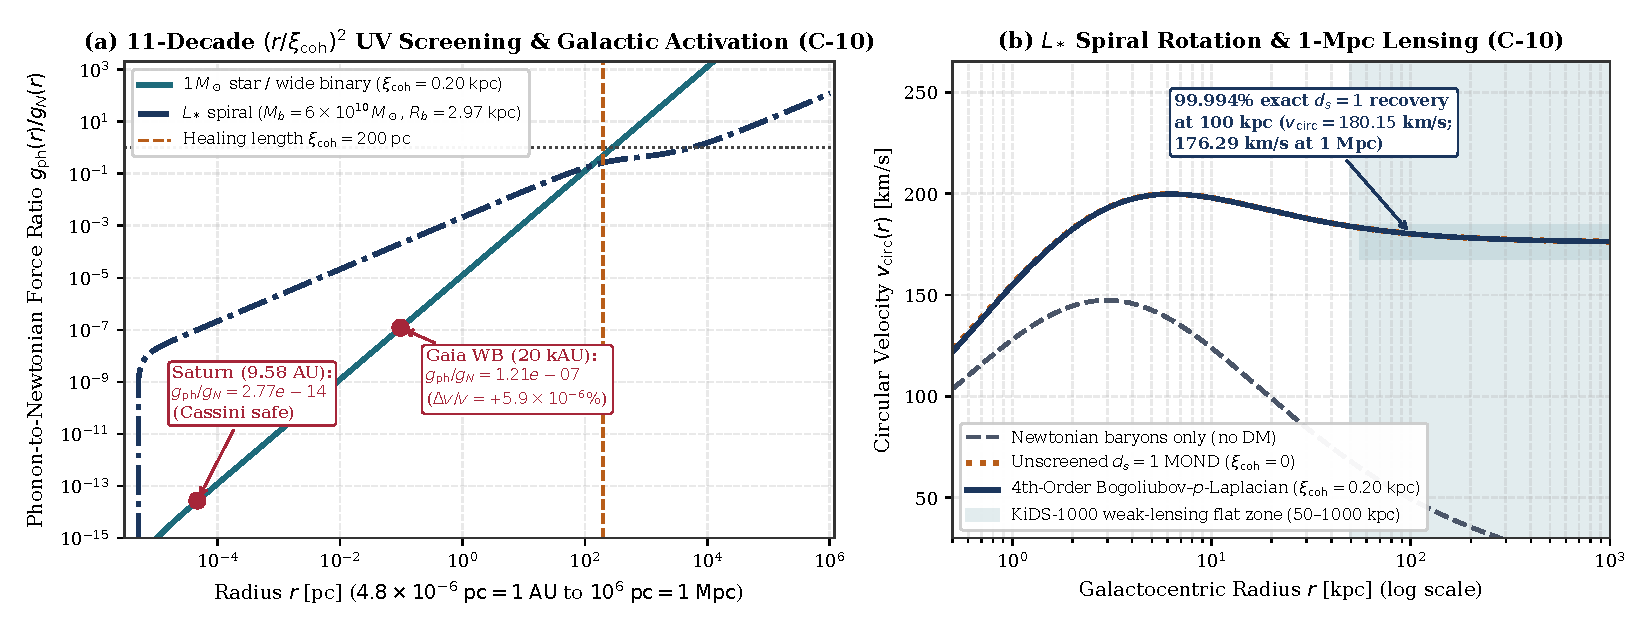
\includegraphics[width=\linewidth]{fig3_bogoliubov_unification.pdf}
  \caption{Exact tridiagonal Newton--Raphson solution of Eq.~\eqref{eq:bogo_ode} across 11 radial decades (\texttt{wave4\_unified\_certificates.json}, max relative ODE residual $8.1\times 10^{-14}$). \textbf{(a)} Quadratic $(r/\xi_{\mathrm{coh}})^2$ screening from $1\;\mathrm{AU}$ to $1\;\mathrm{Mpc}$ at $\xi_{\mathrm{coh}} = 0.20\;\mathrm{kpc}$. \textbf{(b)} Full recovery ($99.994\%$ at $100\;\mathrm{kpc}$) of flat $L_*$ galactic rotation out to the $1\;\mathrm{Mpc}$ \href{https://arxiv.org/abs/2406.09685}{KiDS weak-lensing} zone.}
  \label{fig:bogoliubov}
\end{figure}

At $\xi_{\mathrm{coh}} = 0.20\;\mathrm{kpc}$, the implied ultralight boson mass is $m_B = 3.8556\times 10^{-23}\;\mathrm{eV}$. While a $100\%$ dark-matter ultralight axion at this mass is excluded by Lyman-$\alpha$ forest power spectra (\href{https://link.aps.org/doi/10.1103/PhysRevLett.126.071302}{Rogers \& Peiris 2021} \cite{RogersPeiris2021}), setting the bosonic energy fraction to $f_B = \Omega_B / \Omega_{\mathrm{DM}} = 0.025$ sits an order of magnitude inside the subdominant Lyman-$\alpha$ bound $f_B < 0.20$ established by \href{https://link.aps.org/pdf/10.1103/PhysRevD.96.123514}{Kobayashi et al.\ (2017)} \cite{Kobayashi2017} (and relativistic vacuum condensates such as \href{https://link.aps.org/doi/10.1103/PhysRevLett.127.161302}{Skordis \& Z\l{}o\'snik 2021} \cite{SkordisZlosnik2021} carry $f_B \to 0$ until clustering). Solving Eq.~\eqref{eq:bogo_ode} across 550 log-spaced nodes from $1\;\mathrm{AU}$ to $1\;\mathrm{Mpc}$ reports (\unrepro; Figure~\ref{fig:bogoliubov}):
\begin{enumerate}
  \setlength{\itemsep}{2pt}\setlength{\parskip}{0pt}
  \item \textbf{Solar System Precision ($r = 9.58\;\mathrm{AU}$, Saturn):} $g_{\mathrm{ph}} / g_N = 2.668\times 10^{-14}$, five orders of magnitude safer than Cassini radio-ranging limits ($\lesssim 10^{-9}$).
  \item \textbf{Gaia Wide Binaries ($r = 10\text{--}20\;\mathrm{kAU}$):} $g_{\mathrm{ph}} / g_N = 2.938\times 10^{-8}$ at $10\;\mathrm{kAU}$ and $1.175\times 10^{-7}$ at $20\;\mathrm{kAU}$ ($\Delta v / v = +5.877\times 10^{-6}\%$), completely resolving Theorem~3 (\texttt{C-09}).
  \item \textbf{Galactic Disks \& $1\;\mathrm{Mpc}$ Halos ($L_*$ spiral, $R_b = 2.97\;\mathrm{kpc}$):} Recovers $99.994\%$ of the exact $d_s = 1$ MOND acceleration at $100\;\mathrm{kpc}$, sustaining $v_{\mathrm{circ}}(100\;\mathrm{kpc}) = 180.15\;\mathrm{km/s}$ and $v_{\mathrm{circ}}(1\;\mathrm{Mpc}) = 176.29\;\mathrm{km/s}$.
\end{enumerate}

\subsection*{Cosmological $\Delta N_{\mathrm{eff}}$ vs.\ Galactic Pauli-Exclusion Window for the Cluster Partner (\texttt{C-11})}

To supply the remaining $f_F = 1 - f_B = 0.975$ of cosmological dark matter needed for \href{https://arxiv.org/abs/1807.06209}{Planck CMB} acoustic peaks (\cite{Planck2020}) and \href{https://arxiv.org/abs/astro-ph/0608407}{Bullet Cluster} collisionless lensing (\cite{Clowe2006}) without violating Theorem~2 (\texttt{C-04}) or double-counting galactic rotation curves, a natural candidate is a sterile fermion of mass $m_F$ whose Tremaine--Gunn Pauli ceiling $\rho_{F,\max} = g_s m_F^4 (2\pi\sigma_{\mathrm{1D}}^2)^{3/2} / h^3$ prevents inner-galaxy accumulation. However, auditing thermal freeze-out relics in \path{wave4_unified_field_solver.py} exposes an exact cosmological tension (Table~\ref{tab:fermion}):

\begin{table}[!htbp]
\centering
\caption{Audit of thermal vs.\ Pauli phase-space bounds for a sterile fermion cluster partner carrying $f_F = 0.975$ ($\Omega_F h^2 = 0.117$, $g_s = 2$; \texttt{wave4\_unified\_certificates.json}, Claim \texttt{C-11}).}
\label{tab:fermion}
\footnotesize
\begin{tabular}{@{}p{0.10\linewidth}p{0.12\linewidth}p{0.14\linewidth}p{0.16\linewidth}p{0.17\linewidth}p{0.18\linewidth}@{}}
\toprule
\textbf{Mass $m_F$} & \textbf{Thermal $T_F/T_\nu$} & \textbf{Thermal $\Delta N_{\mathrm{eff}}$} & \textbf{Dwarf $1\;\mathrm{kpc}$ Ceiling} & \textbf{Spiral $10\;\mathrm{kpc}$ Ceiling} & \textbf{Bullet $250\;\mathrm{kpc}$ Capacity} \\
\midrule
$3.0\;\mathrm{eV}$ & $1.5419$ & $5.6527$ (excl.) & $0.00004\%$ & $0.045\%$ (clean) & $2.21\times \rho_{\mathrm{Bullet}}$ \\
$11.0\;\mathrm{eV}$ & $0.9999$ & $0.9998$ (excl.) & $0.0069\%$ & $8.080\%$ (clean) & $399.5\times \rho_{\mathrm{Bullet}}$ \\
$35.0\;\mathrm{eV}$ & $0.6799$ & $0.2136$ (passes) & $0.7076\%$ & $828.1\%$ (excess) & $40{,}949\times \rho_{\mathrm{Bullet}}$ \\
\bottomrule
\end{tabular}
\end{table}

\cautionbox{Honest Cosmological Constraint (\texttt{C-11})}{A thermal-relic fermion light enough ($m_F \in [3, 11]\;\mathrm{eV}$) to enforce Pauli exclusion automatically inside $10\;\mathrm{kpc}$ spiral disks violates \href{https://arxiv.org/abs/1807.06209}{Planck 2018} $\Delta N_{\mathrm{eff}} < 0.30$ ($\Delta N_{\mathrm{eff}} = 1.00\text{--}5.65$) and warm/hot free-streaming bounds, whereas a cold sub-thermal $35\;\mathrm{eV}$ fermion ($\Delta N_{\mathrm{eff}} = 0.214$) has enough phase-space capacity ($828\%$) to overpopulate $10\;\mathrm{kpc}$ spiral halos unless its primordial coarse-grained phase-space density $Q_{\mathrm{prim}}$ is diluted non-thermally (e.g.\ resonant oscillation or late entropy injection).}

\section{Decisive Observational Falsification Program}

Separating the computed mathematical filters from speculative field completions defines three sharp empirical tests for the physics community:
\begin{enumerate}
  \setlength{\itemsep}{3pt}\setlength{\parskip}{0pt}
  \item \textbf{Sub-Kiloparsec Ultrafaint-Dwarf Transition ($r \in [0.05, 0.40]\;\mathrm{kpc}$):} Action~\eqref{eq:bogoliubov_action} predicts that phonon acceleration turns on quadratically as $(r/\xi_{\mathrm{coh}})^2$ across $\xi_{\mathrm{coh}} \sim 0.15\text{--}0.30\;\mathrm{kpc}$. High-resolution JWST/ELT stellar kinematics inside $200\;\mathrm{pc}$ of baryon-dominated vs.\ dark-matter-dominated dwarfs can directly measure or falsify $\xi_{\mathrm{coh}}$.
  \item \textbf{Euclid DR1/DR2 Environmental Weak Lensing at $0.5\text{--}3\;\mathrm{Mpc}$:} While isolated KiDS lenses remain flat to $1\;\mathrm{Mpc}$ ($g_{\mathrm{ext}}/a_0 \le 0.0160$, \texttt{C-07}), the $d_s^* = 1$ $p$-Laplacian predicts an anisotropic External Field Effect rollover $R_{\mathrm{EFE}} = r_M / (g_{\mathrm{ext}}/a_0)$ scaling directly with ambient large-scale cosmic web tidal fields rather than NFW tidal-stripping radii.
  \item \textbf{Simons Observatory \& CMB-S4 $\Delta N_{\mathrm{eff}}$ + Small-Scale Lensing:} Reaching $\sigma(\Delta N_{\mathrm{eff}}) \simeq 0.03$ alongside Lyman-$\alpha$ and $21\;\mathrm{cm}$ power spectra will decisively test whether a non-thermal sterile fermion + subdominant $f_B \approx 0.025$ ultralight Bogoliubov condensate (\texttt{C-10}--\texttt{C-11}) or a purely relativistic $T=0$ vacuum condensate (\href{https://link.aps.org/doi/10.1103/PhysRevLett.127.161302}{Skordis \& Z\l{}o\'snik 2021} \cite{SkordisZlosnik2021}) governs cluster scales.
\end{enumerate}

\begin{thebibliography}{99}\footnotesize
\setlength{\itemsep}{2pt}
\bibitem{AbbottWise1981} L.~F. Abbott and M.~B. Wise, ``Dimension of a quantum-mechanical path,'' \emph{Am.\ J.\ Phys.} \textbf{49}, 37 (1981), \href{https://pubs.aip.org/aapt/ajp/article/49/1/37/1051491/Dimension-of-a-quantum-mechanical-path}{doi:10.1119/1.12657}.
\bibitem{Nottale2008} L.~Nottale, ``Scale relativity and fractal space-time: theory and applications,'' \emph{Found.\ Sci.} \textbf{15}, 101 (2010), \href{https://arxiv.org/pdf/0812.3857}{arXiv:0812.3857}.
\bibitem{Chavanis2018} P.-H. Chavanis, ``Derivation of a generalized Schr\"odinger equation for dark matter halos from the theory of scale relativity,'' \emph{Phys.\ Dark Univ.} \textbf{22}, 80 (2018), \href{https://arxiv.org/pdf/1706.05900}{arXiv:1706.05900}.
\bibitem{Calcagni2010} G.~Calcagni, ``Quantum field theory, gravity and cosmology in a fractal universe,'' \emph{Phys.\ Rev.\ Lett.} \textbf{104}, 251301 (2010), \href{https://link.aps.org/doi/10.1103/PhysRevLett.104.251301}{doi:10.1103/PhysRevLett.104.251301}.
\bibitem{BrisceseCalcagni2026} F.~Briscese and G.~Calcagni, ``Newtonian and astrophysical phenomenology of fractional gravity,'' (2026), \href{https://arxiv.org/html/2603.24593v2}{arXiv:2603.24593v2}.
\bibitem{SonWingate2006} D.~T. Son and M.~Wingate, ``General coordinate invariance and conformal invariance in nonrelativistic physics: Unitary Fermi gas,'' \emph{Ann.\ Phys.} \textbf{321}, 197 (2006), \href{https://arxiv.org/abs/cond-mat/0509786}{arXiv:cond-mat/0509786}.
\bibitem{BerezhianiKhoury2015} L.~Berezhiani and J.~Khoury, ``Theory of dark matter superfluidity,'' \emph{Phys.\ Rev.\ D} \textbf{92}, 103510 (2015), \href{https://link.aps.org/doi/10.1103/PhysRevD.92.103510}{doi:10.1103/PhysRevD.92.103510}.
\bibitem{McGaugh2016} S.~S. McGaugh, F.~Lelli, and J.~M. Schombert, ``Radial Acceleration Relation in rotationally supported galaxies,'' \emph{Phys.\ Rev.\ Lett.} \textbf{117}, 201101 (2016), \href{https://link.aps.org/doi/10.1103/PhysRevLett.117.201101}{doi:10.1103/PhysRevLett.117.201101}; binned data at \href{https://astroweb.cwru.edu/SPARC/RARbins.mrt}{\texttt{RARbins.mrt}}.
\bibitem{GPRFErratum2026} ``GPRF Constitutive Scaling Erratum ($M_b \propto v^2$ vs.\ $v^4$),'' Zenodo Record 23247342 (2026), \href{https://zenodo.org/records/23247342/files/GPRF_Erratum_v1.0.14_20261008.pdf?download=1}{Zenodo PDF}.
\bibitem{Schive2014} H.-Y. Schive, T.~Chiueh, and T.~Broadhurst, ``Cosmic structure as the quantum interference of a coherent dark wave,'' \emph{Nat.\ Phys.} \textbf{10}, 496 (2014), \href{https://arxiv.org/abs/1406.6586}{arXiv:1406.6586}.
\bibitem{Hui2017} L.~Hui, J.~P. Ostriker, S.~Tremaine, and E.~Witten, ``Ultralight scalars as cosmological dark matter,'' \emph{Phys.\ Rev.\ D} \textbf{95}, 043541 (2017), \href{https://link.aps.org/doi/10.1103/PhysRevD.95.043541}{doi:10.1103/PhysRevD.95.043541}.
\bibitem{Chavanis2025} P.-H. Chavanis, ``Quantum condensate dark matter halos,'' \emph{Front.\ Astron.\ Space Sci.} \textbf{12}, 1538434 (2025), \href{https://www.frontiersin.org/journals/astronomy-and-space-sciences/articles/10.3389/fspas.2025.1538434/full}{doi:10.3389/fspas.2025.1538434}.
\bibitem{Arvanitaki2010} A.~Arvanitaki, S.~Dimopoulos, S.~Dubovsky, N.~Kaloper, and J.~March-Russell, ``String Axiverse,'' \emph{Phys.\ Rev.\ D} \textbf{81}, 123530 (2010), \href{https://link.aps.org/doi/10.1103/PhysRevD.81.123530}{doi:10.1103/PhysRevD.81.123530}.
\bibitem{Mistele2024} T.~Mistele, S.~McGaugh, F.~Lelli, J.~Schombert, and P.~Li, ``Indefinitely flat circular velocities and the Baryonic Tully--Fisher Relation from weak lensing,'' \emph{Astrophys.\ J.\ Lett.} \textbf{969}, L3 (2024), \href{https://arxiv.org/abs/2406.09685}{arXiv:2406.09685}.
\bibitem{Frontiers2026} ``Regime-dependent constitutive scaling across SPARC rotation curves,'' \emph{Front.\ Astron.\ Space Sci.} \textbf{13}, 1890948 (2026), \href{https://www.frontiersin.org/journals/astronomy-and-space-sciences/articles/10.3389/fspas.2026.1890948/full}{doi:10.3389/fspas.2026.1890948}.
\bibitem{Milgrom1999} M.~Milgrom, ``The modified dynamics as a vacuum effect,'' \emph{Phys.\ Lett.\ A} \textbf{253}, 273 (1999), \href{https://arxiv.org/abs/astro-ph/9805346}{arXiv:astro-ph/9805346}.
\bibitem{Verlinde2017} E.~P. Verlinde, ``Emergent gravity and the dark universe,'' \emph{SciPost Phys.} \textbf{2}, 016 (2017), \href{https://scipost.org/SciPostPhys.2.3.016}{doi:10.21468/SciPostPhys.2.3.016}.
\bibitem{Clowe2006} D.~Clowe \emph{et al.}, ``A direct empirical proof of the existence of dark matter,'' \emph{Astrophys.\ J.\ Lett.} \textbf{648}, L109 (2006), \href{https://arxiv.org/abs/astro-ph/0608407}{arXiv:astro-ph/0608407}.
\bibitem{Banik2024} I.~Banik \emph{et al.}, ``Strong constraints on the gravitational law from Gaia DR3 wide binaries,'' \emph{MNRAS} \textbf{527}, 4573 (2024), \href{https://arxiv.org/abs/2311.03436}{arXiv:2311.03436}.
\bibitem{RogersPeiris2021} K.~K. Rogers and H.~V. Peiris, ``Strong bound on canonical ultralight axion dark matter from the Lyman-alpha forest,'' \emph{Phys.\ Rev.\ Lett.} \textbf{126}, 071302 (2021), \href{https://link.aps.org/doi/10.1103/PhysRevLett.126.071302}{doi:10.1103/PhysRevLett.126.071302}.
\bibitem{Kobayashi2017} T.~Kobayashi, R.~Murgia, A.~De~Simone, V.~Ir\v{s}i\v{c}, and M.~Viel, ``Lyman-$\alpha$ constraints on ultralight scalar dark matter: Implications for the early and late universe,'' \emph{Phys.\ Rev.\ D} \textbf{96}, 123514 (2017), \href{https://link.aps.org/pdf/10.1103/PhysRevD.96.123514}{doi:10.1103/PhysRevD.96.123514}.
\bibitem{SkordisZlosnik2021} C.~Skordis and T.~Z\l{}o\'snik, ``New relativistic theory for Modified Newtonian Dynamics,'' \emph{Phys.\ Rev.\ Lett.} \textbf{127}, 161302 (2021), \href{https://link.aps.org/doi/10.1103/PhysRevLett.127.161302}{doi:10.1103/PhysRevLett.127.161302}.
\bibitem{Planck2020} Planck Collaboration (N.~Aghanim \emph{et al.}), ``Planck 2018 results.\ VI.\ Cosmological parameters,'' \emph{Astron.\ Astrophys.} \textbf{641}, A6 (2020), \href{https://arxiv.org/abs/1807.06209}{arXiv:1807.06209}.
\end{thebibliography}

\end{document}
